\documentclass{article}
\usepackage{graphicx}
\usepackage{hyperref}
\usepackage{listings}
\usepackage{xcolor}
\usepackage{geometry}
\geometry{a4paper, margin=0.8in}
\setlength{\parindent}{0pt}
\setlength{\parskip}{0.8em}

\title{Spreadsheet System Design Report}
\author{Vani Gupta (2023CS10126) \and Neelkanth Mishra (2023CS10022) \and Soubhagya Mohapatra (2023EE31148)}

\begin{document}

\maketitle

\section{Introduction}
This report describes the design and working of our spreadsheet system, built for the command line. The system supports basic arithmetic, functions like SUM, MIN, MAX, and tracks dependencies between cells to keep everything updated automatically.

\section{Design Decisions}
\begin{itemize}
    \item \textbf{Graph-Based Dependencies:} Every cell is a node. Edges show which cells depend on which, making updates easy to track.
    \item \textbf{Linked List Adjacency Lists:} We use linked lists to store dependencies efficiently without wasting memory.
    \item \textbf{Modular Code:} The code is split into clear sections—display handling, parsing, formulas, and graph management.
    \item \textbf{Error Handling:} We handle bad inputs and block circular dependencies to keep the system stable.
    \item \textbf{Memory Management:} We allocate and free memory carefully to handle large spreadsheets smoothly.
\end{itemize}

\section{Challenges Faced}

\begin{itemize}
    \item \textbf{Cycle Detection:} Avoiding infinite loops from circular references between cells.
    \item \textbf{Memory Usage:} Handling big spreadsheets without slowing down.
    \item \textbf{Formula Parsing:} Parsing and understanding complex expressions accurately.
    \item \textbf{User Interface:} Making navigation and control smooth in a terminal-based environment.
    \item \textbf{Live Updates:} Ensuring dependent cells always show the latest correct values.
\end{itemize}

\section{Program Structure}
\begin{itemize}
    \item \textbf{1.c:} The main program that handles inputs and runs the spreadsheet.
    \item \textbf{display.c/h:} Controls how the spreadsheet looks in the terminal and handles scrolling.
    \item \textbf{Functions.c/h:} Contains functions like SUM, MIN, MAX, AVERAGE, and others.
    \item \textbf{Graph.c/h:} Manages the dependency graph and checks for cycles.
    \item \textbf{Parser.c/h:} Breaks down user commands and runs the right operations.
    \item \textbf{Makefile:} Automates building and testing the project.
\end{itemize}
\section{Data Structures Used}

\begin{itemize}
    \item \textbf{Graph (Adjacency List):} 
    Each cell is a node, and its dependencies are stored as linked lists. This makes adding, deleting, and traversing dependencies efficient.
    
    \item \textbf{Linked Lists:} 
    Used in the adjacency list to manage dependencies for each cell without extra memory overhead.

    \item \textbf{Range List:} 
    For functions like SUM, MIN, MAX over cell ranges, we store ranges as a linked list of range nodes. Each range keeps track of its start and end cells and which cell depends on that range.

    \item \textbf{Formula Array:} 
    An array that stores the formula or operation for each cell. It tracks what kind of operation the cell holds and which cells or constants it uses.

    \item \textbf{Integer Array (Spreadsheet Data):} 
    The actual values of the spreadsheet are stored in a flat integer array, with cells indexed based on row and column.

    \item \textbf{DFS/Recursion Stack Arrays:} 
    Temporary arrays are used for depth-first search (DFS) during cycle detection and topological sorting.
\end{itemize}
\section{Test Suite}
\subsection{Test Coverage}
\begin{itemize}
    \item \textbf{Basic Value Assignments:} Verifying that constant values can be assigned to cells and are stored correctly.
    \item \textbf{Arithmetic Operations:} Validating calculations involving two operands (like addition, subtraction, multiplication, and division) with combinations of constants and cell references.
    \item \textbf{Functions:} Ensuring functions like SUM, MIN, MAX, AVERAGE, and STDEV operate correctly over specified ranges.
    \item \textbf{Range Validations:} Testing boundary cases of ranges, invalid ranges, and out-of-bounds access.
    \item \textbf{Cycle Detection:} Confirming that cycles are correctly detected, rejected, and that previous stable states are restored.
    \item \textbf{Dependency Propagation:} Verifying that updates propagate properly to all dependent cells when a referenced cell is modified.
    \item \textbf{Error Handling:} Ensuring the system responds appropriately to invalid commands, invalid cell references, division by zero, and other error cases.
\end{itemize}

\subsection{Test Implementation}
\begin{itemize}
    \item Tests are written within \texttt{Tests.c}.
    \item The tests use predefined sequences of inputs to simulate user interactions and check the state of the spreadsheet after each command.
    \item Assertions are made on cell values to confirm expected outputs.
    \item Edge cases are stressed, such as large range calculations, negative numbers, and sequential updates.
\end{itemize}

\subsection{Running the Tests}
The test suite is integrated with the build system and can be executed using:
\begin{lstlisting}
make test
\end{lstlisting}
This will compile the program and execute all test cases, providing pass/fail results in the terminal.


\section{Algorithms}

\subsection{Dependency Updates}
When you change a cell, every cell that depends on it needs to be updated too. Here's how we handle that:
\begin{itemize}
    \item We use DFS (Depth-First Search) starting from the changed cell to find all affected cells.
    \item We build a topological order of these cells so that no cell gets updated before the ones it depends on.
    \item Finally, we recalculate each cell in this order to update the whole chain properly.
\end{itemize}
\begin{figure}[h]
    \centering
    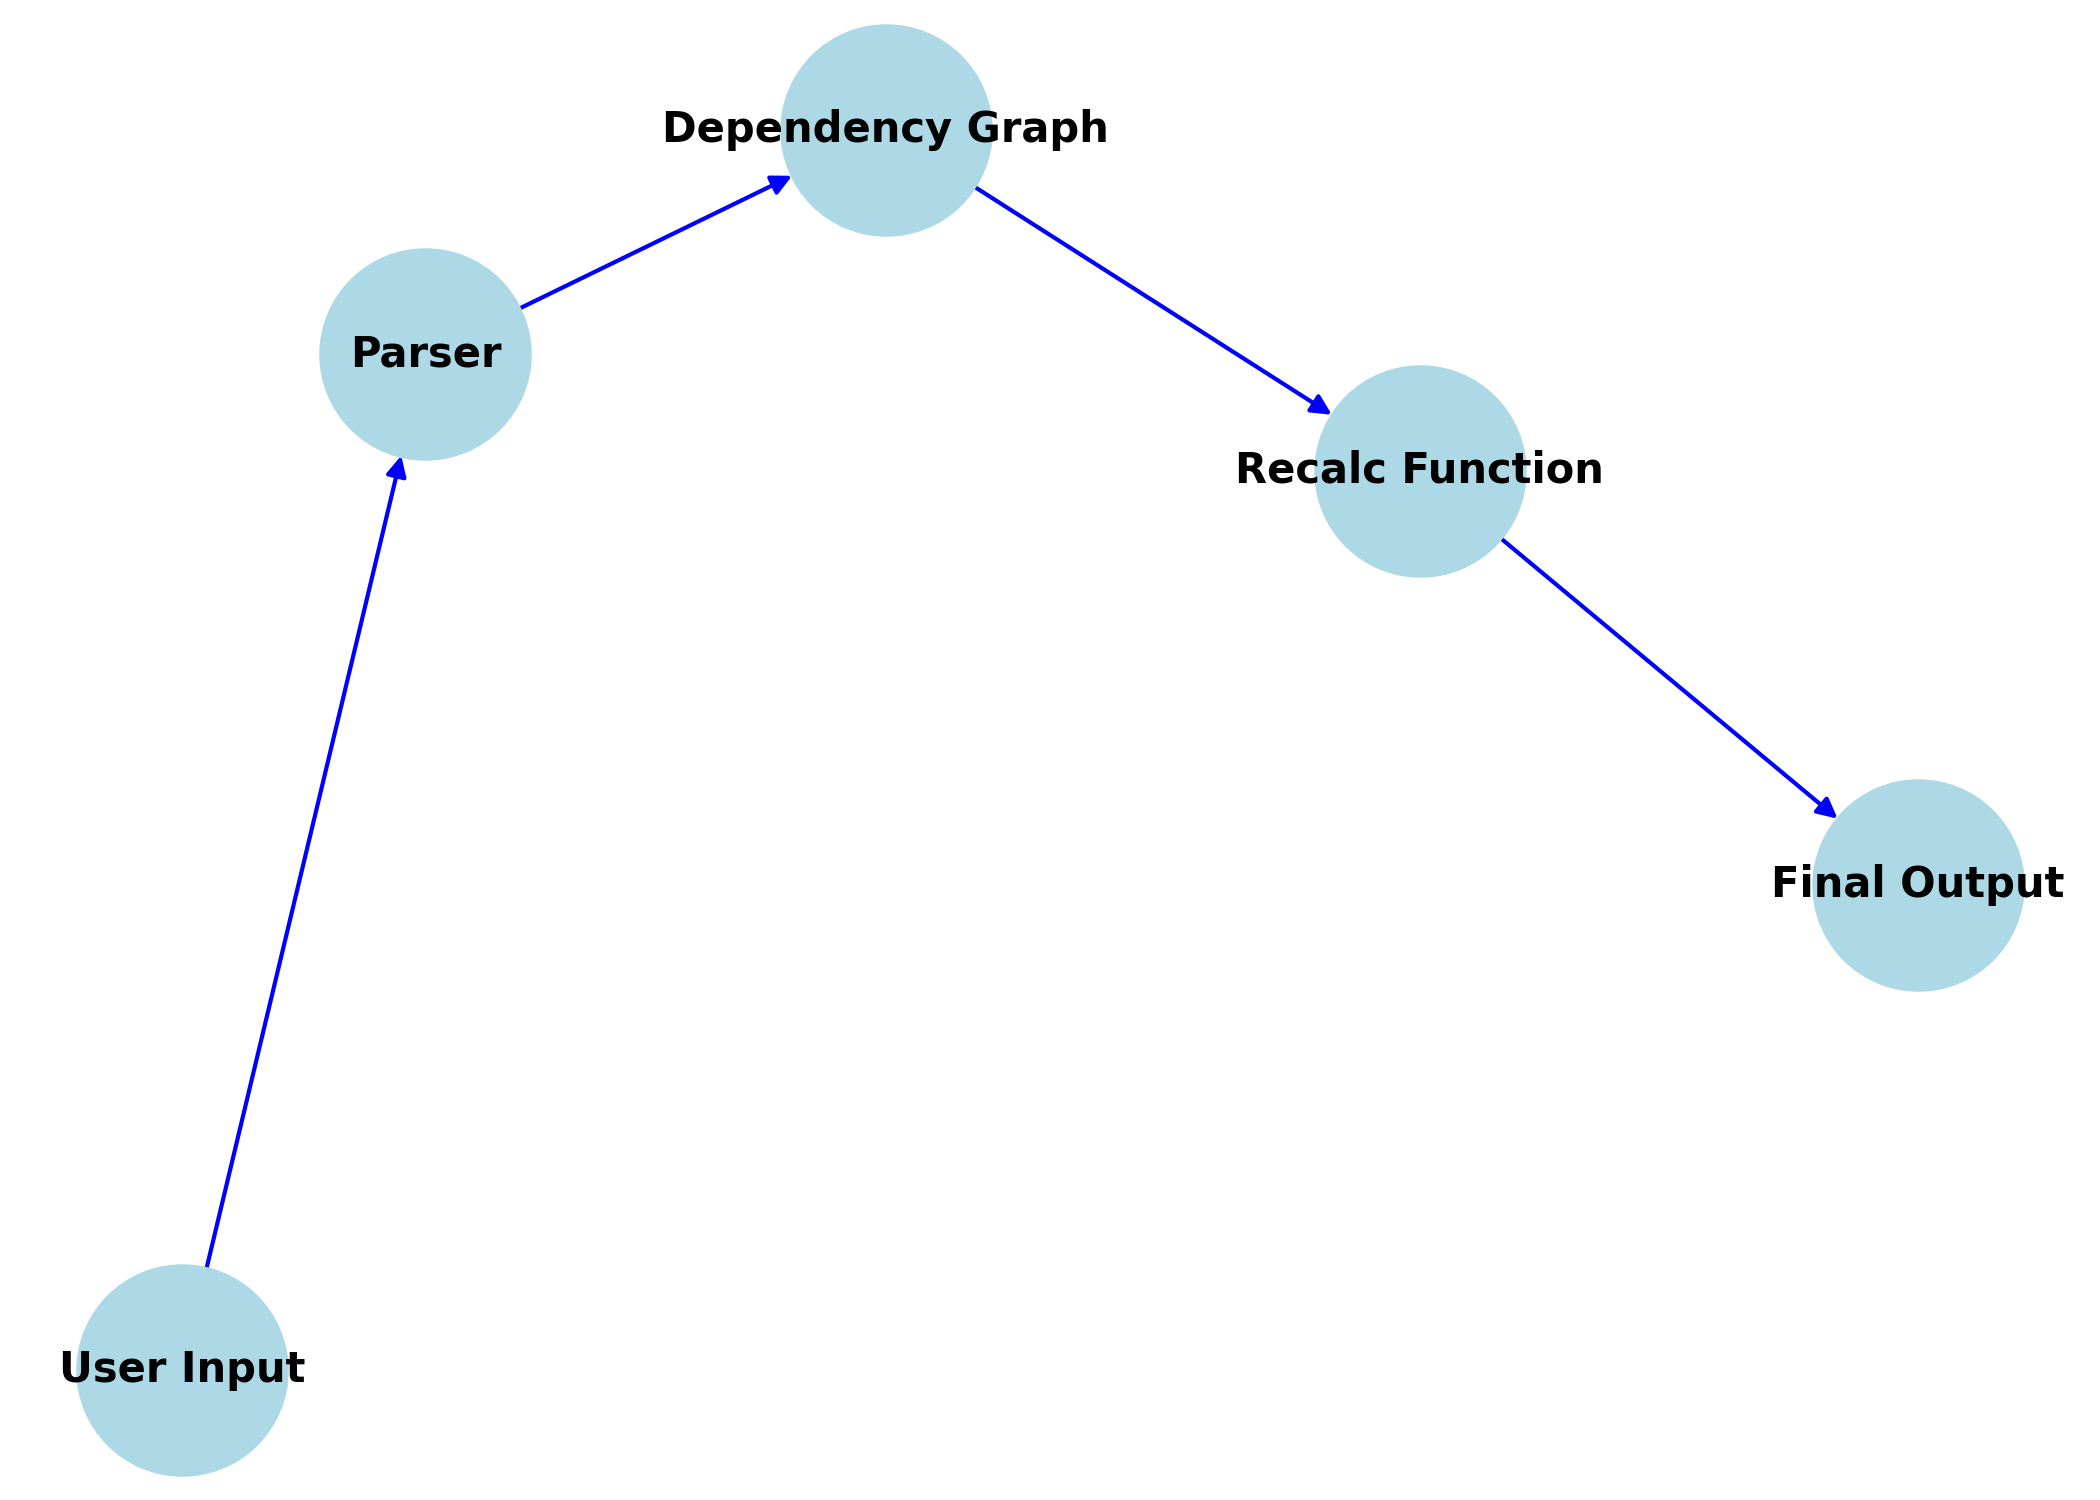
\includegraphics[width=0.4\textwidth]{data_flow.png}
    \caption{Data Flow in the Spreadsheet}
\end{figure}

\subsection{Cycle Detection}
We must ensure there are no loops (cycles) where cells depend on each other forever. Here's how we check:
\begin{itemize}
    \item We run a DFS whenever formulas are updated.
    \item If we find that we revisit a cell while still on the same DFS path, that’s a cycle.
    \item If a cycle is found, we cancel the operation and tell the user.
\end{itemize}
\begin{figure}[h]
    \centering
    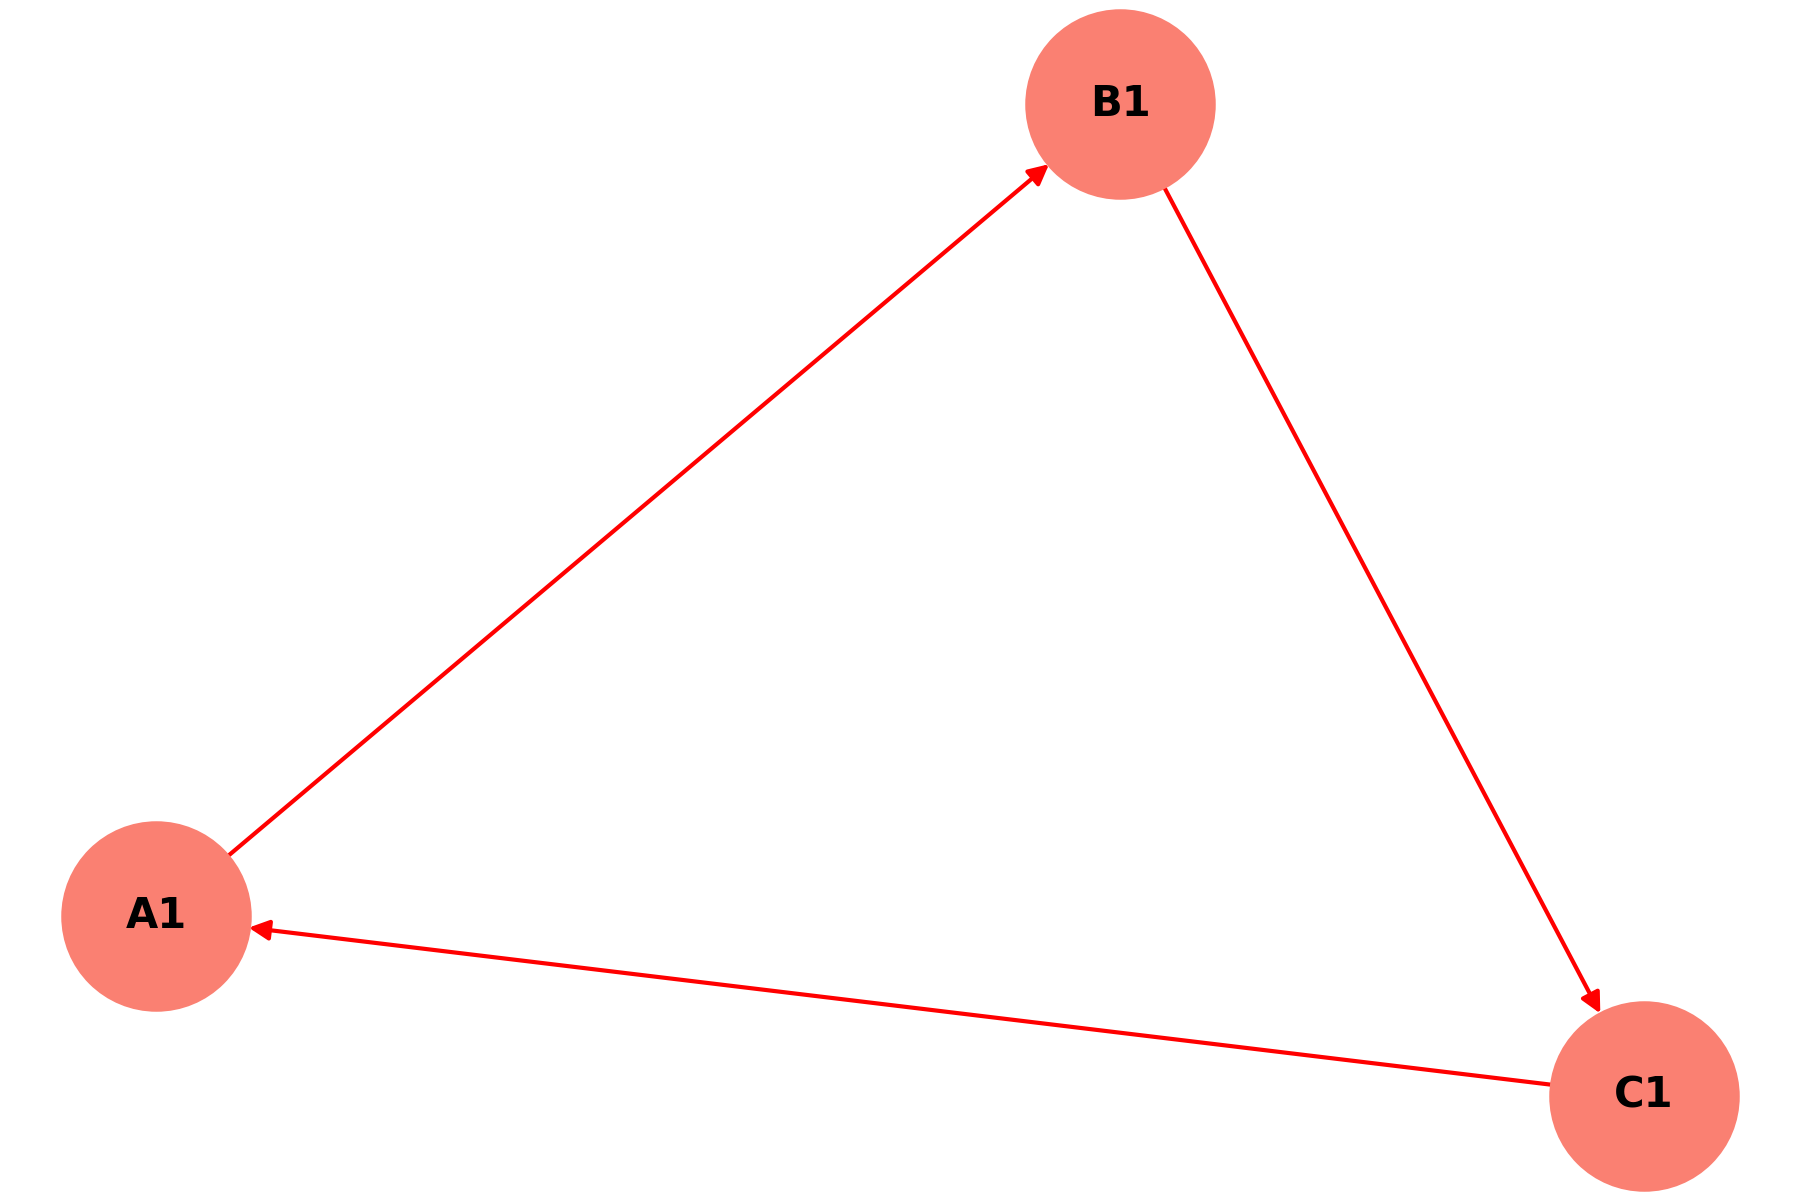
\includegraphics[width=0.4\textwidth]{cycle_detection.png}
    \caption{Cycle Detection Mechanism}
\end{figure}

\subsection{Topological Sorting}
To update cells in the right order:
\begin{itemize}
    \item We use DFS to explore all cells affected by a change.
    \item As we finish visiting cells, we add them to a list in reverse order.
    \item This list gives us the correct order to update cells without missing dependencies.
\end{itemize}
\begin{figure}[h]
    \centering
    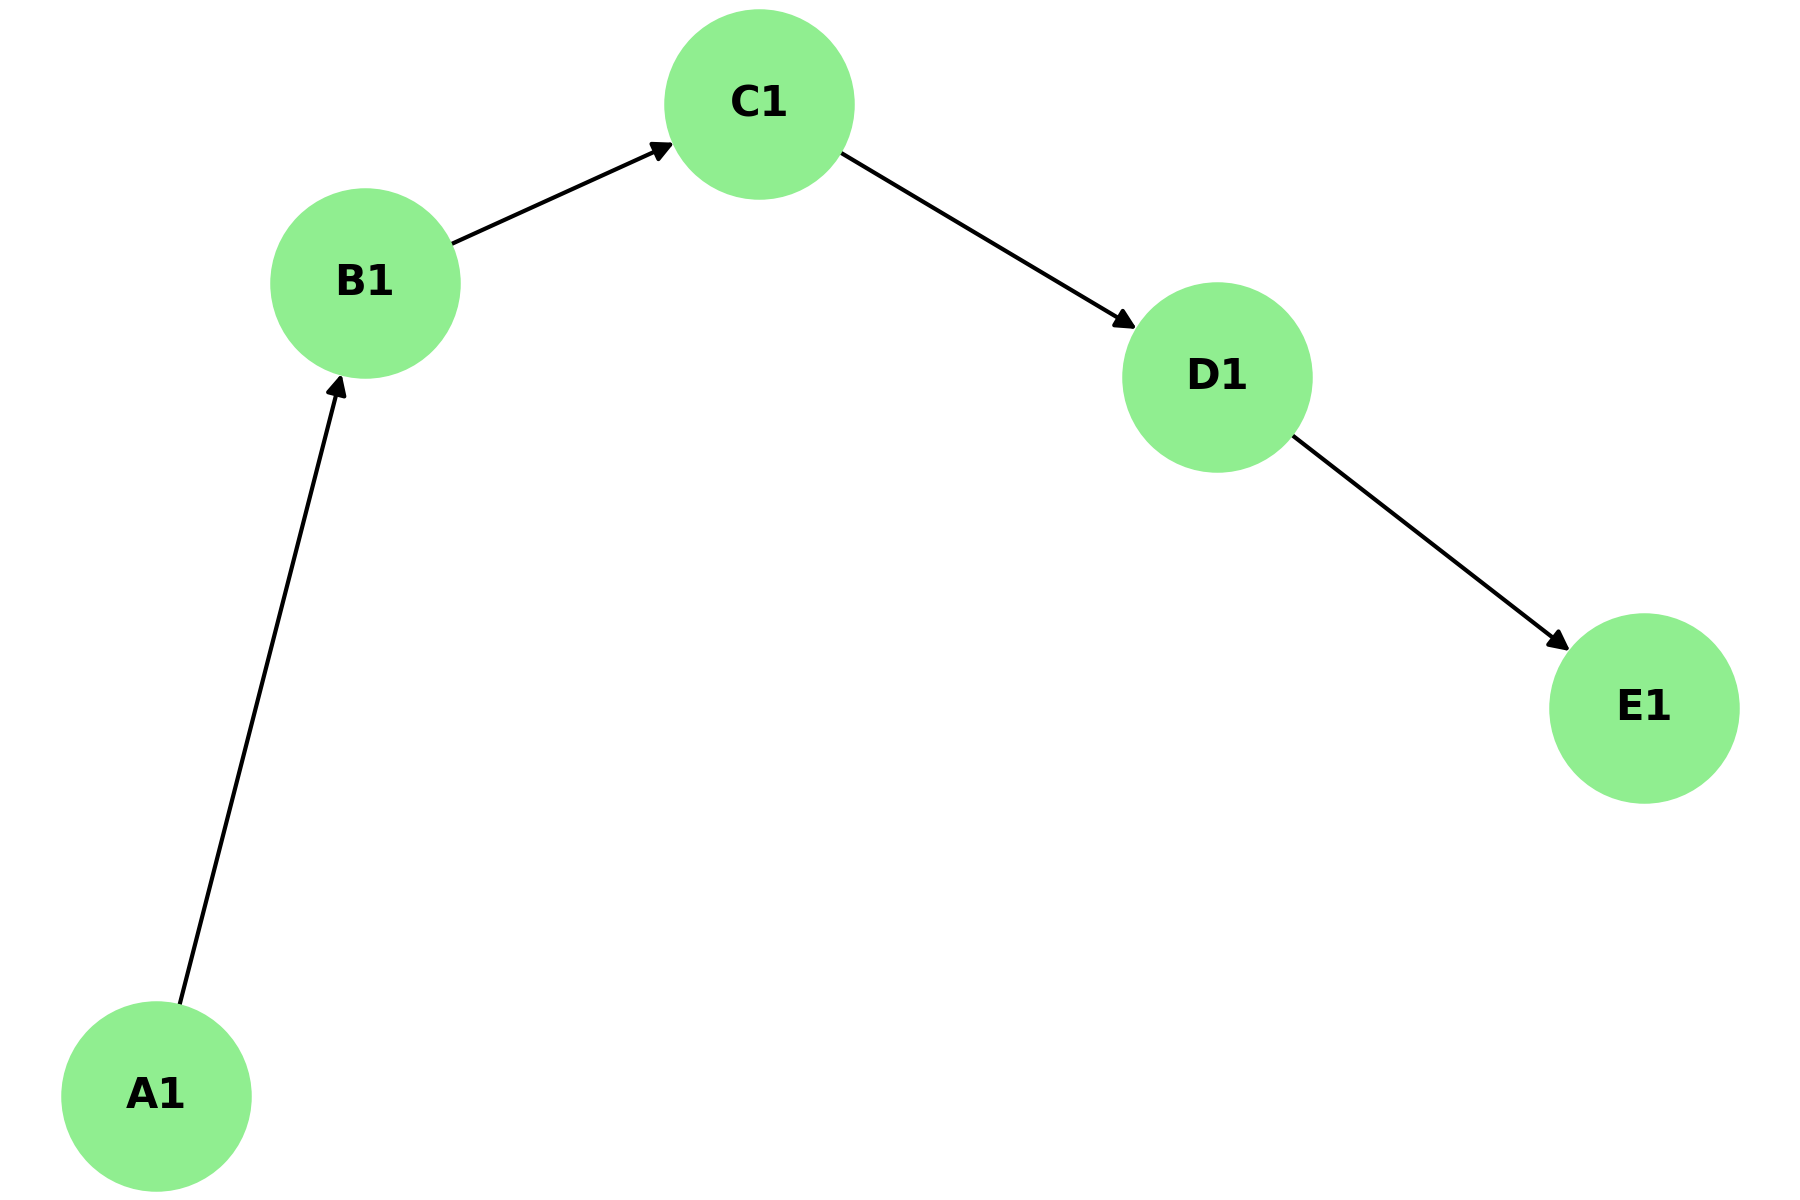
\includegraphics[width=0.4\textwidth]{topological_sorting.png}
    \caption{Topological Sorting}
\end{figure}

\section{Build and Run}
To compile and run the program:
\begin{lstlisting}
make        # Build the program
make test   # Run test cases
./spreadsheet 10 10  # Start a 10x10 spreadsheet
\end{lstlisting}

\section{Conclusion}
Our spreadsheet system successfully manages dynamic updates, formulas, and dependencies while staying responsive in the terminal. Future improvements could include:
\begin{itemize}
    \item Adding a graphical user interface (GUI).
    \item Supporting more advanced statistical functions.
    \item Improving performance for very large spreadsheets.
    \item Adding multithreading to speed up heavy computations.
\end{itemize}

\section{Resources}
\textbf{Demo Video}: \href{https://example.com/demo}{Watch Here}\\
\textbf{GitHub Repository}: \href{https://github.com/example/repo}{View Here}

\end{document}
